\documentclass[letterpaper,10pt]{article}

\usepackage{titling}
\usepackage{listings}
\usepackage{url}
\usepackage{setspace}
\usepackage{subfig}
\usepackage{sectsty}
\usepackage{pdfpages}
\usepackage{colortbl}
\usepackage{multirow}
\usepackage{relsize}
\usepackage{amsmath}
\usepackage{fancyvrb}
\usepackage{amsmath,amssymb,amsthm,graphicx,xspace}
\usepackage[titlenotnumbered,noend,noline]{algorithm2e}
\usepackage[compact]{titlesec}
\usepackage[default]{droidserif}
\usepackage[T1]{fontenc}
\usepackage{tikz}
\usetikzlibrary{arrows,automata,shapes,trees,matrix,chains,scopes,positioning,calc}
\tikzstyle{block} = [rectangle, draw, fill=blue!20, 
    text width=2.5em, text centered, rounded corners, minimum height=2em]
\tikzstyle{bw} = [rectangle, draw, fill=blue!20, 
    text width=4em, text centered, rounded corners, minimum height=2em]

\definecolor{namerow}{cmyk}{.40,.40,.40,.40}
\definecolor{namecol}{cmyk}{.40,.40,.40,.40}

\let\LaTeXtitle\title
\renewcommand{\title}[1]{\LaTeXtitle{\textsf{#1}}}


\newcommand{\handout}[5]{
  \noindent
  \begin{center}
  \framebox{
    \vbox{
      \hbox to 5.78in { {\bf ECE155: Engineering Design with Embedded Systems } \hfill #2 }
      \vspace{4mm}
      \hbox to 5.78in { {\Large \hfill #4  \hfill} }
      \vspace{2mm}
      \hbox to 5.78in { {\em #3 \hfill} }
    }
  }
  \end{center}
  \vspace*{4mm}
}

\newcommand{\lecture}[3]{\handout{#1}{#2}{#3}{Lecture #1}}
\newcommand{\tuple}[1]{\ensuremath{\left\langle #1 \right\rangle}\xspace}

\addtolength{\oddsidemargin}{-1.000in}
\addtolength{\evensidemargin}{-0.500in}
\addtolength{\textwidth}{2.0in}
\addtolength{\topmargin}{-1.000in}
\addtolength{\textheight}{1.75in}
\addtolength{\parskip}{\baselineskip}
\setlength{\parindent}{0in}
\renewcommand{\baselinestretch}{1.5}
\newcommand{\term}{Spring 2014}

\singlespace


\begin{document}

\lecture{ 1 --- Introduction to Embedded Systems}{\term}{Jeff Zarnett, based on original by Patrick Lam}

\section*{About the Course}
We'll start by reviewing the highlights of the class syllabus. Please read it carefully (it is available in Learn). It contains a lot of important information about the class including: the lecture topics, the grading scheme, contact information for the course staff, and university policies.

\section*{Introduction to Embedded Systems}

\begin{quote}
    \emph{A general-purpose definition of embedded systems is that they
      are devices used to control, monitor or assist the operation of
      equipment, machinery or plant. ``Embedded'' reflects the fact that
      they are an integral part of the system. In many cases, their
      ``embeddedness'' may be such that their presence is far from
      obvious to the casual observer. Even the more technically skilled
      might need to examine the operation of a piece of equipment for
      some time before being able to conclude that an embedded control
      system was involved in its functioning.}
\end{quote}
\hfill(Institute of Electrical Engineers)

Where can you find embedded systems?

\begin{itemize}
	\item Cellphones/other communications systems
	\item Microwaves/thermostats/other appliances
	\item Industrial automation
	\item Medical devices
	\item Transportation: aviation and automobiles
\end{itemize}

\paragraph{Two types of embedded systems.} The term \textit{embedded system}
covers many systems. Simple embedded systems might be constructed out of electronics without a processor or control software. Complex embedded systems incorporate one or more processors along with control software.

Another term is \textit{embedded computer system}, which overlaps with
complex embedded systems. We'll call an embedded computer system a special-purpose computer system designed to perform a set of tasks without the user's knowledge of its existence.


\paragraph{Example: Exhaust Gas Recirculator}
Many vehicles have a device in the engine called the Exhaust Gas Recirculator (EGR).
\begin{itemize}
	\item \emph{Problem:} car engines produce oxides of nitrogen (NOx) when they burn too hot. 
	\item \emph{Solution:} The best way to do that is to recirculate
already-burned exhaust gases, which don't burn again, thus lowering the
temperature.
	\item \emph{When?} It's difficult to figure this out. Hence, embedded
systems.
\end{itemize}

Mechanically, the EGR contains a valve which lets exhaust gases back
into the combustion chamber.
% draw a picture

\begin{center}
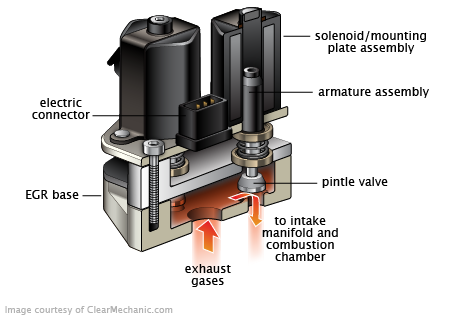
\includegraphics[width=0.75\textwidth]{images/egrvalve.png}
\hfill \url{http://repairpal.com/exhaust-gas-recirculation-system}
\end{center}

\paragraph{First Approach.} When you step on the gas, this opens, and
then closes, the EGR valve. However, you don't need, or want, EGR on a
cold engine, because it lowers the engine's performance. So, GM put a
fully-mechanical thermal switch in its cars. Unfortunately, this
didn't work well, because mechanical components often don't work the
way you want them to, as you'll find out.

\paragraph{More Mechanical Components.} Car manufacturers added more
components, like vacuum amplifiers, delay valves, and solenoids, to
fix the issues: ``spaghetti'' tubes.

\paragraph{Embedded Systems in EGRs.} Today's solution is to use a
small embedded system to control the EGR valve. 

What are the inputs and outputs of the EGR system?
\\[1em]
Inputs: RPM, throttle, temperature (sensors)\\
Outputs: signal to the valve; pulse-width modulation (actuators)

\paragraph{Design Constraints.} There are two main constraints when
choosing which processors (or electronics) to include in your embedded
system.

\begin{itemize}
\item Processor power: The processor must be able to crunch
enough bits. In particular, it needs to have good enough latency (response
time) and bandwidth (processing power) to control the systems it's
responsible for. Plus, you need to be able to model its performance
characteristics.
\item Environment: You have to be able to embed the processor. In particular,
you have to respect size, power and connectivity constraints.
\end{itemize}

\paragraph{Challenges.} Beyond meeting the design constraints, it's harder
to write code for embedded systems than for PCs for a few additional
reasons:

\begin{itemize}
\item Variability: Programming Windows systems is all the same, while
programming cellphones is quite different from programming EGRs.
\item No/bad UI: Can't necessarily put a print statement into a 
microwave oven's embedded system, nor can you put it in the state
you'd want to.
\item No API: An embedded system might not contain any operating system
to speak of.
\item Hard to get at: Have to load the software onto the system,
which can be hard.
\end{itemize}

\paragraph{Block Diagram.} Here are some parts of a typical
embedded system.

\begin{center}
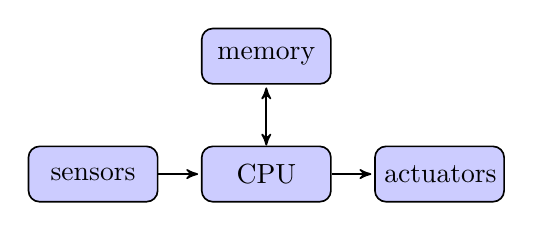
\begin{tikzpicture}[->,>=stealth',shorten >=1pt,auto,node distance=2.2cm,
                    semithick,initial text=]
  \node[bw]   (cpu)               {CPU};
  \node[bw, left of=cpu] (sensors) {sensors};
  \node[bw, right of=cpu] (actuators) {actuators};
  \node[bw, above of=cpu,yshift=-2em] (memory) {memory};

  \path (cpu) edge[<->] node {} (memory)
        (sensors) edge node {} (cpu)
        (cpu) edge node {} (actuators);
\end{tikzpicture}
\end{center}
Sensors provide input to the CPU, while actuators enable the CPU
to affect the outside world.

\section*{Sensors and Actuators}
Embedded systems differ from general-purpose computers in that their
interaction with the outside world is much more important than in a
general-purpose computer.


\subsection*{Sensors} Sensors convert input from the external environment
into a form suitable for use by a computer system.

Most phenomena in the outside world are analog and continuous-time,
while the computer is digital and discrete-time, so something has to
convert between these realms.

For instance, a light sensor might represent intensity as an
analog voltage, while the computer needs a stream of bits.

\paragraph{Analog-to-Digital Converters.} To go between the realms,
use an {\bf ADC}, which converts a continuous-time analog signal into a
discrete-time digital signal.

The conversion is approximate, and loses information if the samples are
too infrequent\footnote{See the Nyquist sampling theorem.} or if the
samples don't capture enough information (i.e. their resolution is too poor).

\begin{center}
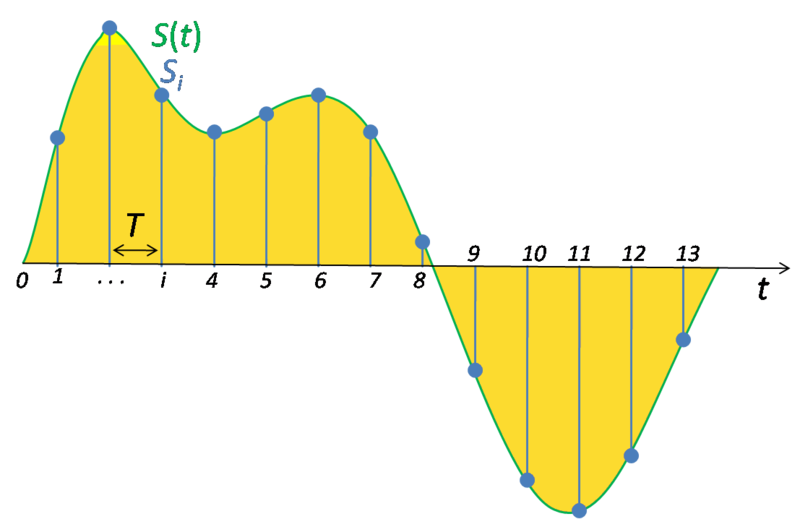
\includegraphics[width=0.5\textwidth]{images/sampling.png}
\hfill \url{http://en.wikipedia.org/wiki/File:Signal_Sampling.png}
\end{center}

Note that the digital signal is a finite set of pairs, each of which
contains a sample and a time for that sample.

\paragraph{Actuators.} Actuators convert output from the computer
system into some effect on the environment.  What are some
  examples of actuators?

motors, LCDs, LEDs, heaters/AC units, potentiometer, speakers

Some actuators require analog voltage signals. In those cases, you
have to feed the discrete-time data to a digital-to-analog converter
({\bf DAC}).

\paragraph{Combined Sensors and Actuators.} Of course, we can combine
sensing and actuating in a single device. Some devices automatically
do this, like piezoelectric sensors. Any relatively modern game
controller also combines sensors and actuators, particularly the Wii
Remote. Phones also combine sensors and actuators.


\section*{Programming the Embedded System}
We'll discuss how to program the CPU next. Programming an embedded
system is somewhat similar to programming a computer, but there are
differences in the programming environment and in the structure of the
code.
We run an \emph{embedded control program} on an embedded system, e.g. a modem. It monitors
sensor inputs and controls actuators. Some embedded computer systems use an embedded operating system to manage devices and run embedded applications.  Such systems behave much like a general-purpose computer.  For example, a cellular phone might run an embedded operating system that allows a user to start and terminate applications.

Let's talk first about the structure of the code. Embedded control programs:
\begin{itemize}
\item boot automatically on device power up;
\item never terminate under normal use;
\item process a stream of inputs and outputs; and
\item care about timing.
\end{itemize}

Embedded control programs may run on top of embedded operating systems.
An \emph{embedded operating system} is a special type of operating system designed for use in embedded computer systems; it has these properties:
\begin{itemize}
\item is compact and efficient;
\item cares about battery life;
\item provides APIs between devices and application software; and
\item favours portability.
\end{itemize}

\subsection*{Therac-25}
The Therac-25 cancer radiation therapy machine is one of the most famous cases of engineering failure. It's referenced in practically every book about software failures, engineering books, and so on. This is especially the case where the authors or intended audience are Canadian, because the machine was developed by Atomic Energy of Canada Limited. Three patients died as a result of the many problems with the system \cite{spos}:

\begin{itemize}
	\item \textbf{Race Condition}: A race condition existed between the operator interface task and the equipment control task. This did not occur in testing because AECL did not expect that operators would enter commands in such a quick succession. As operators became more proficient with the system, they entered the commands faster.
	\item \textbf{Overflow}: A flag was incremented and an overflow caused the software to bypass the normal safety checks.
	\item \textbf{Interlocks}: The maximum power setting was enabled without the thick metal plate being in place.
	\item \textbf{Incorrect Feedback}: Although patients had received a fatal amount of radiation, the machine showed that the machine had not delivered the prescribed dose, causing operators to deliver another dose.
\end{itemize}


Someone has to build these embedded systems, and lives, including yours, will depend on them.

\subsection*{Collaborative Course}
The source material for the ECE~155 notes and slides is now open-sourced via Github (\url{http://www.github.com}), an online collaboration tool. Later on we will learn about \texttt{git}, but if you're already familiar with it, so much the better. Whether or not you know how to use \texttt{git}, if you find an error in the notes/slides, or have an idea on how to improve them, go to \url{https://github.com/jzarnett/ece155} and open an issue. 

If you know how to use \texttt{git} and \LaTeX, then you can go to the URL and submit a pull request (changes) for me to look at and incorporate!

\bibliographystyle{alpha}
\bibliography{155}


\end{document}